\title{\it Mergesort}
\frame{\maketitle}

\begin{frame}{\inserttitle}
  \begin{itemize}
  \item Algoritmo de divisão e conquista.
    \begin{description}
    \item[Divisão] Divide o vetor original em tamanhos menores.
    \item[Conquista] Mescla ({\em merge}) estes subvetores menores,
      ordenando-os, até obter um vetor do tamanho do original com todos 
      os elementos ordenados.
    \end{description}
  \end{itemize}
\end{frame}

\begin{frame}[fragile]{Fase da conquista}{\tt merge()}
  \lstinputlisting[firstline=2,lastline=16]{../sort/merge.c}
\end{frame}

\begin{frame}[fragile]{Fase da divisão}{\tt mergesort()}
  \lstinputlisting[firstline=17]{../sort/merge.c}
\end{frame}

\begin{frame}{{\tt mergesort()}--fase da divisão}
  
  \begin{center}
    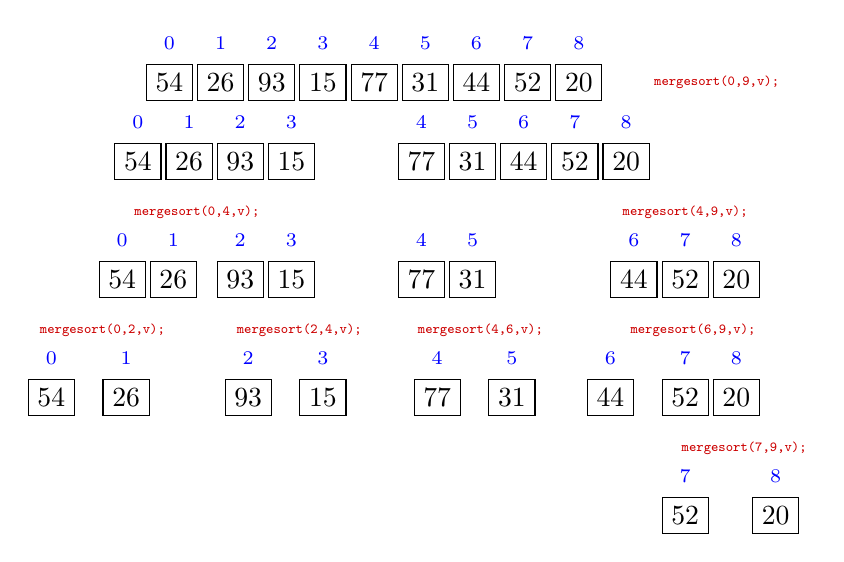
\begin{tikzpicture}[idx/.style={font=\scriptsize,blue},
      val/.style={minimum width=2cm},
      callfunc/.style={font=\tt\tiny,red!80!black,xshift=.75cm}
      ]
      % 1st phase
      \foreach \i/\v in {0/54,1/26,2/93,3/15,4/77,5/31,6/44,7/52,8/20} {
        \node<1->[idx] (i1\i) at (.65*\i,0) {\i};
        \node<1->[below of=i1\i,yshift=.5cm,draw] (v1\i) {\v};
      }
      \node<1->[callfunc,right of=v18] {mergesort(0,9,v);};
      
      % 2nd phase
      \foreach \i/\v in {0/54,1/26,2/93,3/15} {
        \node<2->[idx] (i2\i) at (-.4+.65*\i,-1cm) {\i};
        \node<2->[below of=i2\i,yshift=.5cm,draw] (v2\i) {\v};
      }
      \foreach \i/\v in {4/77,5/31,6/44,7/52,8/20} {
        \node<2->[idx] (i2\i) at (.6+.65*\i,-1cm) {\i};
        \node<2->[below of=i2\i,yshift=.5cm,draw] (v2\i) {\v};
      }

      % 3rd phase
      \node<3->[callfunc,below of=v20,yshift=.35cm] {mergesort(0,4,v);};
      \node<3->[callfunc,below of=v28,yshift=.35cm] {mergesort(4,9,v);};
      \foreach \i/\v in {0/54,1/26} {
        \node<4->[idx] (i3\i) at (-.6+.65*\i,-2.5cm) {\i};
        \node<4->[below of=i3\i,yshift=.5cm,draw] (v3\i) {\v};
      }

      \foreach \i/\v in {2/93,3/15} {
        \node<4->[idx] (i3\i) at (-.4+.65*\i,-2.5cm) {\i};
        \node<4->[below of=i3\i,yshift=.5cm,draw] (v3\i) {\v};
      }

      \foreach \i/\v in {4/77,5/31} {
        \node<4->[idx] (i3\i) at (.6+.65*\i,-2.5cm) {\i};
        \node<4->[below of=i3\i,yshift=.5cm,draw] (v3\i) {\v};
      }
      \foreach \i/\v in {6/44,7/52,8/20} {
        \node<4->[idx] (i3\i) at (2+.65*\i,-2.5cm) {\i};
        \node<4->[below of=i3\i,yshift=.5cm,draw] (v3\i) {\v};
      }

      % 4rd phase
      \node<5->[callfunc,below of=v30,yshift=.35cm,xshift=-1cm] {mergesort(0,2,v);};
      \node<5->[callfunc,below of=v32,yshift=.35cm] {mergesort(2,4,v);};
      \node<5->[callfunc,below of=v34,yshift=.35cm] {mergesort(4,6,v);};
      \node<5->[callfunc,below of=v36,yshift=.35cm] {mergesort(6,9,v);};
      \foreach \i/\v in {0/54} {
        \node<6->[idx] (i4\i) at (-1.5+.65*\i,-4cm) {\i};
        \node<6->[below of=i4\i,yshift=.5cm,draw] (v4\i) {\v};
      }

      \foreach \i/\v in {1/26} {
        \node<6->[idx] (i4\i) at (-1.2+.65*\i,-4cm) {\i};
        \node<6->[below of=i4\i,yshift=.5cm,draw] (v4\i) {\v};
      }
      
      \foreach \i/\v in {2/93} {
        \node<6->[idx] (i4\i) at (-.3+.65*\i,-4cm) {\i};
        \node<6->[below of=i4\i,yshift=.5cm,draw] (v4\i) {\v};
      }
      \foreach \i/\v in {3/15} {
        \node<6->[idx] (i4\i) at (.65*\i,-4cm) {\i};
        \node<6->[below of=i4\i,yshift=.5cm,draw] (v4\i) {\v};
      }
      
      \foreach \i/\v in {4/77} {
        \node<6->[idx] (i4\i) at (.8+.65*\i,-4cm) {\i};
        \node<6->[below of=i4\i,yshift=.5cm,draw] (v4\i) {\v};
      }

      \foreach \i/\v in {5/31} {
        \node<6->[idx] (i4\i) at (1.1+.65*\i,-4cm) {\i};
        \node<6->[below of=i4\i,yshift=.5cm,draw] (v4\i) {\v};
      }

      \foreach \i/\v in {6/44} {
        \node<6->[idx] (i4\i) at (1.7+.65*\i,-4cm) {\i};
        \node<6->[below of=i4\i,yshift=.5cm,draw] (v4\i) {\v};
      }
      
      \foreach \i/\v in {7/52,8/20} {
        \node<6->[idx] (i4\i) at (2+.65*\i,-4cm) {\i};
        \node<6->[below of=i4\i,yshift=.5cm,draw] (v4\i) {\v};
      }

      % 5rd phase
      \node<7->[callfunc,below of=v47,yshift=.35cm] {mergesort(7,9,v);};
      \foreach \i/\v in {7/52} {
        \node<8->[idx] (i4\i) at (2+.65*\i,-5.5cm) {\i};
        \node<8->[below of=i4\i,yshift=.5cm,draw] (v4\i) {\v};
      }

      \foreach \i/\v in {8/20} {
        \node<8->[idx] (i4\i) at (2.5+.65*\i,-5.5cm) {\i};
        \node<8->[below of=i4\i,yshift=.5cm,draw] (v4\i) {\v};
      }       
    \end{tikzpicture}
  \end{center}
\end{frame}


\begin{frame}{{\tt merge()}--fase da conquista}
  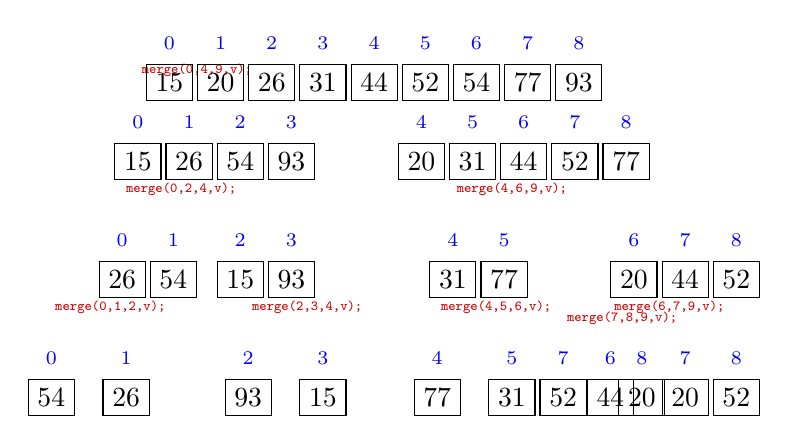
\begin{tikzpicture}[idx/.style={font=\scriptsize,blue},
    val/.style={minimum width=2cm},
    callfunc/.style={font=\tt\tiny,red!80!black,xshift=.75cm}
    ]
    
    \node at (0,0) (O) {};
    % 
    \foreach \i/\v in {7/52} {
      \node<1>[idx,below of=O,xshift=5cm,yshift=-3cm] (i\i) {\i};
      \node<1>[below of=i\i,yshift=.5cm,draw] (v\i) {\v};
    }

    \foreach \i/\v in {8/20} {
      \node<1>[idx,right of=i7] (i\i) {\i};
      \node<1>[below of=i\i,yshift=.5cm,draw] (v\i) {\v};
    }
    \node<1>[callfunc,above of=i7,yshift=-.5cm] {merge(7,8,9,v);};

    % 
    \foreach \i/\v in {0/54} {
      \node<2,3>[idx] (i\i) at (-1.5+.65*\i,-4cm) {\i};
      \node<2,3>[below of=i\i,yshift=.5cm,draw] (v\i) {\v};
    }

    \foreach \i/\v in {1/26} {
      \node<2,3>[idx] (i\i) at (-1.2+.65*\i,-4cm) {\i};
      \node<2,3>[below of=i\i,yshift=.5cm,draw] (v\i) {\v};
    }
    
    \foreach \i/\v in {2/93} {
      \node<2,3>[idx] (i\i) at (-.3+.65*\i,-4cm) {\i};
      \node<2,3>[below of=i\i,yshift=.5cm,draw] (v\i) {\v};
    }
    \foreach \i/\v in {3/15} {
      \node<2,3>[idx] (i\i) at (.65*\i,-4cm) {\i};
      \node<2,3>[below of=i\i,yshift=.5cm,draw] (v\i) {\v};
    }
    
    \foreach \i/\v in {4/77} {
      \node<2,3>[idx] (i\i) at (.8+.65*\i,-4cm) {\i};
      \node<2,3>[below of=i\i,yshift=.5cm,draw] (v\i) {\v};
    }

    \foreach \i/\v in {5/31} {
      \node<2,3>[idx] (i\i) at (1.1+.65*\i,-4cm) {\i};
      \node<2,3>[below of=i\i,yshift=.5cm,draw] (v\i) {\v};
    }

    \foreach \i/\v in {6/44} {
      \node<2,3>[idx] (i\i) at (1.7+.65*\i,-4cm) {\i};
      \node<2,3>[below of=i\i,yshift=.5cm,draw] (v\i) {\v};
    }
    
    \foreach \i/\v in {7/20,8/52} {
      \node<2,3>[idx] (i\i) at (2+.65*\i,-4cm) {\i};
      \node<2,3>[below of=i\i,yshift=.5cm,draw] (v\i) {\v};
    }
    \node<3>[callfunc,above of=i0,yshift=-.35cm] {merge(0,1,2,v);};
    \node<3>[callfunc,above of=i2,yshift=-.35cm] {merge(2,3,4,v);};
    \node<3>[callfunc,above of=i4,yshift=-.35cm] {merge(4,5,6,v);};
    \node<3>[callfunc,above of=i6,yshift=-.35cm] {merge(6,7,9,v);};
    % 
    \foreach \i/\v in {0/26,1/54} {
      \node<4,5>[idx] (i\i) at (-.6+.65*\i,-2.5cm) {\i};
      \node<4,5>[below of=i\i,yshift=.5cm,draw] (v\i) {\v};
    }

    \foreach \i/\v in {2/15,3/93} {
      \node<4,5>[idx] (i\i) at (-.4+.65*\i,-2.5cm) {\i};
      \node<4,5>[below of=i\i,yshift=.5cm,draw] (v3\i) {\v};
    }

    \foreach \i/\v in {4/31,5/77} {
      \node<4,5>[idx] (i\i) at (1+.65*\i,-2.5cm) {\i};
      \node<4,5>[below of=i\i,yshift=.5cm,draw] (v\i) {\v};
    }
    \foreach \i/\v in {6/20,7/44,8/52} {
      \node<4,5>[idx] (i\i) at (2+.65*\i,-2.5cm) {\i};
      \node<4,5>[below of=i\i,yshift=.5cm,draw] (v\i) {\v};
    }
    \node<5>[callfunc,above of=i0,yshift=-.35cm] {merge(0,2,4,v);};
    \node<5>[callfunc,above of=i4,yshift=-.35cm] {merge(4,6,9,v);};

    % 
    \foreach \i/\v in {0/15,1/26,2/54,3/93} {
      \node<6,7>[idx] (i\i) at (-.4+.65*\i,-1cm) {\i};
      \node<6,7>[below of=i\i,yshift=.5cm,draw] (v\i) {\v};
    }
    \foreach \i/\v in {4/20,5/31,6/44,7/52,8/77} {
      \node<6,7>[idx] (i\i) at (.6+.65*\i,-1cm) {\i};
      \node<6,7>[below of=i\i,yshift=.5cm,draw] (v\i) {\v};
    }
    \node<7>[callfunc,above of=i0,yshift=-.35cm] {merge(0,4,9,v);};

    \foreach \i/\v in {0/15,1/20,2/26,3/31,4/44,5/52,6/54,7/77,8/93} {
      \node<8>[idx] (i\i) at (.65*\i,0) {\i};
      \node<8>[below of=i\i,yshift=.5cm,draw] (v\i) {\v};
    }
  \end{tikzpicture}
\end{frame}

\begin{frame}{Ordem de complexidade}{Desempenho}
  \Large
  \begin{equation*}
    O(nlog_2n)
  \end{equation*}

\end{frame}

\begin{frame}{Referência}
  \begin{thebibliography}{9}
  \bibitem{feofiloff2008} Paulo Feofiloff, \\
    {\em Algoritmos em linguagem C}.\\
    Editora Campus, 2008-2009.\\
    \href{http://www.ime.usp.br/~pf/algoritmos/aulas/mrgsrt.html}{Página web do mesmo autor sobre mergesort}.
  \end{thebibliography}

\end{frame}

%% 
% Local variables:
% TeX-master: main
% End:
%% 